In order to describe the experiments that I've conducted in the context of this thesis, two general aspects have to be covered: one, common for all the experiments conducted, concerns the tools that I used, as well as the specific pipeline that I developed, in order to be able to conduct such experiments. This will be the focus of the present chapter.\\
The other aspect, specific for each experiment, concerns the motivations that led to every specific experiment, together with a description of the settings, architectures and results involved, as well as the interpretation of the results that led to subsequent experiments. This will be discussed in chapter \ref{experiments}.\\

Note that the following general considerations apply to the whole chapter:
\begin{itemize}
\item All the Python scripts can be found under the https://github.com/andres-fr/bachelor-thesis/code/ link.
\item The data and the labels can be found under the https://github.com/andres-fr/bachelor-thesis/datasets/ link.
\item The computer language used for the development of the whole project is \texttt{Python 2.7}.
\end{itemize}



\section{Data Downloading and Storage}

As described in chapter \ref{about-ds}, the curators of the carnatic corpus developed and kindly granted us access to Dunya, an open-source platform that provides a web service as well as a Python API for accessing the labels and recordings needed to conduct the experiments. The source files, together with a description of their usage can be found in the following GitHub link: \url{https://github.com/MTG/dunya}.\\

The API function \texttt{get\_recordings()} provides a list of unique IDs, that can be used to access each recording as an mp3 file, and its label as a dictionary of unicode strings. See the Python scripts \texttt{1\_download\_carnatic.py} and \texttt{2\_download\_metadata\\.py} in the \texttt{code} folder for more details.\\

The downloaded data is stored as \texttt{HDF5} (a binary data format that allows storage of huge amounts of numerical data), via the \texttt{h5py} Python package\cite{h5py}, which is allows to ``easily manipulate HDF5 data from NumPy''\cite{h5py}. \texttt{NumPy} is ``the fundamental package for scientific computing with Python''\cite{numpy}.\\

HDF5 alows different ranges of lossless compression on the stored data, as well as very flexible hashing and indexing of the data chunks. In the Python implementation, it is organized in the form of dictionaries in which the keys are strings and the data are NumPy arrays. The keys can then be grouped into higher-order dictionaries, allowing the creation of tree structures.\\

For a single-label, supervised classification task, this way of organizing the data makes the idea a dictionary of dictionaries (here abbreviated as {\it ddict}) a very natural way to store and structure the downloaded datasets: the higher-ordered dictionary stores the label (in our case the r\=aga's ID) as a key and the lower-ordered dictionary as the corresponding value. And each lower-ordered dictionary stores the sample ID (in our case the recording's ID) as a key and the recording itself as a value. See the fourth section of the \texttt{3\_main\_pipeline.py} Python script for more implementation details.

\section{Data Representation and Preprocessing}

Since deep neural networks perform representation learning, it is difficult to tell where the optimal border between preprocessing and learning is. In this context, it can be observed that ``usually, operations that are generally applicable (such as adding Gaussian noise to the input) are considered part of the machine learning algorithm, while operations that are specific to one application domain (such as randomly cropping an image) are considered to be separate preprocessing steps''\cite[p.242]{goodfellow}. The present thesis follows this approach.

\subsection{Converting mp3 Files to wav}

The development of the mp3 format started in the late 80s at the Fraunhofer IIS in Germany\cite{mp3}. It provides a lossy compression that exploits psychoacoustical phenomena like the {\it masking} (which happens when the perception of one louder sound disallows the perception of other softer sounds) to provide very low bitrates without much loss of the perceived information. Since the details of the compression algorithm are very involved, and I didn't find any literature that performed end-to-end music classification based on mp3 files, I wasn't certain if they would provide a good representation. For this reason I converted them to mono wav files, which have been used extensively (directly or as a basis for other representations) in many recent machine learning setups, as reported in chapter \ref{context}.\\

Wav files contain a discrete representation of the musical waveform along the time domain (in my case 22050 samples per second and 16 bits per sample). The audio conversion was performed using the \texttt{ffmpeg} program. For more details on the implementation, see the third section of the \texttt{3\_main\_pipeline.py} Python script.

\subsection{The Fourier Transform}

This section intends to provide a coverage on the matter sufficient to give an idea of the related preprocessing operations conducted in this project, by putting a focus on the intuition. As general reference for the contents of this chapter, \cite{musimathics} has been consulted, especially chapter 3.\\

A transform is a mathematical operation, ``a way to represent the same information in an equivalent form''. The Fourier transform is, for many reasons, one of the key concepts in the field of Digital Signal Processing (DSP). It is based in the idea that ``any periodic vibration, no matter how complicated it seems, can be built up from sinusoids whse frequencies are integer multiples of a fundamental frequency, by choosing the proper amplitudes and phases''.\\

In other words, the waveform of an audio signal representing the intensity of the signal at a given time point, can be represented as well as a set of sinusoidal functions, without any loss of information. Each sinusoidal would have then three parameters: amplitude, frequency and phase, which are naturally represented by complex numbers (or by a linear combination of a sine and a cosine, as stated by Euler's identity \(e^{i\theta}=cos\theta+i\cdot sin\theta\)). The resulting representation of such amplitude and phase across the frequency domain is known as the spectrum of that signal. Note that, unlike the waveform, the spectrum gives no explicit information about the intensity of the signal at a given time point.


\subsubsection{Analysis}

The process of ``choosing the proper amplitudes and phases'' in order to decompose a signal into a set of sinusoidals is colloquially known as the Fourier transform, but Fourier analysis is the actual name of the operation. Intuitively, it can be seen as a filter bank: given the waveform of a signal, and a set of sinusoidal waves, it ``asks'' to the given signal how compatible is it for every one of the sinusoidals. The ``answer'' for each frequency is this compatibility in the form of an amplitude and a phase. The following equation represents the discrete Fourier transform: for a given discrete waveform \(x(n), n \in \{0, 1,..., N-1\}\), it outputs the corresponding complex component \(X(k)\) of the spectrum for the \(k\) frequency:\\

\begin{equation*}
  \begin{aligned}
    X(k) = \frac{1}{N} \sum_{n=0}^{N-1} \big\{ x(n)e^{-ik2\pi n / N} \big\}
  \end{aligned}
\end{equation*}


Note that \(n\) represents a given time point and \(k\) a given frequency. By looking at the exponent of the complex sinusoidal, it is also possible to develop an intuition for the canonical set of filters that are used to ``ask'': We know from Euler's identity that the codomain of the \(e^{-i2\pi n / N}\) function divides the unit circle into \(N\) evenly distributed values, so, for \(k=1\), this complex signal will draw one whole loop between \(n=0\) and \(n=N-1\). And for \(k=2\), two whole loops, and so on.\\

This way, a lossless spectral representation of the signal can be achieved exactly when \(k \in \{0, 1,..., N-1\}\), and explains the idea that the frequencies of the resulting filter bank are ``integer multiples of the fundamental''. Due to the discrete nature of \(x(n)\), it wouldn't make sense to choose a smaller resolution for \(k\): any transform based on a different set of values for \(k\) could be either equivalent, cause information loss, or be redundant due to aliasing, but never better. Therefore, \(k\) can be intuitively seen as the ``step size'' in samples, and the frequency of the corresponding spectral component will equal \(\frac{k\cdot samplerate}{N}\)Hz.\\

Further, if the signal is real (as in the case of this thesis), the spectrum will be symetrical and only the half of it has to be calculated. In that case, the effective frequency range of the Fourier transform for any real, discrete signal will be between \(0\)Hz and \(\frac{samplerate}{2}\)Hz (the {\it Nyquist frequency}).

\subsubsection{Synthesis}

The Fourier synthesis is the opposite process to the analysis: given a spectrum \(X(k),\; k \in \{0, 1,..., N-1\}\) as a set of amplitudese and phases of complex sinusoidals, reconstruct the waveform \(x(n),\; n \in \{0, 1,..., N-1\}\) . For this reason it is usually referred to as the reverse Fourier transform. The formula resembles the Fourier analysis quite similarly:

\begin{equation*}
  \begin{aligned}
    x(n) = \frac{1}{N} \sum_{k=0}^{N-1} \big\{ X(k)e^{ik2\pi n / N} \big\}

  \end{aligned}
\end{equation*}


Due to this similarity, and knowing the intuition behind the Fourier analyis, understanding this is much easier.\\

First, note that, when multiplying two complex numbers, the phases are added and the magnitudes are multiplied. So the multiplication that happens in the body of the sum is simply capturing the magnitude and the phase for a given spectral component \(X(k)\) by adding its phase to \(ik2\pin/N\) and multiplying its magnitude by 1. But also nothe the following: in the analysis, the complex exponent is negative, whereas here it is positive: when adding them, if the original waveform  \(x(n)\) was real, they will exactly cancel each other resulting in a real signal back again.\\
\\

This way, the waveform \(x(n)\) can be calculated by adding all the spectral components present in \(X(k)\) for a discrete \(n\). At this point it is worth to note why Fourier says ``any periodic vibration'': this reconstruction could be done for any \(x(n), n\in\mathbb{Z}\), but, for a spectrum  \(X(k),\; k \in \{0, 1,..., N-1\}\), the reconstructed signal would repeat itself exactly every \(N\) steps, due to the periodic nature of the sinusoidals themselves, and any information apart from the contained in  \(x(n), n \in \{0, 1,..., N-1\}\) would be redundant.


\subsubsection{Linearity}


One very nice aspect of the Fourier transform is that the process of analysis and synthesis of a signal is linear\cite[p.148]{musimathics}: This means (among many other advantages) numerical stability, computational efficience (the {\it Fast Fourier Transform} (FFT) performs in \(\mathcal{O}(n log(n))\) for a signal of length \(n\)), and that, when performing it within a chain of linear transformations to a signal, the order in which it is performed doesn't alter the result.\\

And this works because any set of complex sinusoidals of \(N\) different frequencies acts as an orthogonal basis for a complex N-dimensional vector space on which any (infinitely periodical) waveform of size \(N\) can be represented. In fact, this idea works for any other family of orthogonal functions: that is the idea behind the Walsh-Hadamard transform (see \cite[p.525]{musimathics} for more details).

\subsubsection{Time/Frequency Tradeoff}

The symmetry between the analysis and the resynthesis process in the Fourier transform is given by the fact that both the \(n\) (representing time) and \(k\) (representing frequency) variables play the exact same functional role: they multiply the exponent of the complex signal. And, since multiplication is commutative, and both variables iterate over the exact same set of natural numbers, they are operationally exchangeable.\\

But not semantically: the fact that both time and frequency domains have the same magnitude doesn't mean that they are identical: for a bigger \(N\), the waveform \(x(n)\) is going to have more duration, and the corresponding frequency range of the spectrum \(X(k)\) will have more frequency bands.\\

Since the spectrum doesn't contain explicit temporal information, and its range is alwayshz distributed in \([0Hz,\; ..., \; samplerate/2)\) for real signals, analyzing a longer signal effectively increases the frequency resolution dicreasing the time resolution proportionally. In other words, it is impossible to have arbitrary precision in both the temporal location and the frequency of a signal's components.\\

  When discussing the quality of a representation, it is usually considered its ability of conveying the relevant information in a convenient and accurate way. In the case of carnatic music, both the temporal and spectral aspects are considered relevant information. The fact that the Fourier transform doesn't provide arbitrary precission in both of them motivated the development of the time-frequency representations discussed in the following section.

  \subsection{Time-Frequency Representations} \label{timefreqrepr}

  Intending to overcome the problem of the time/frequency tradeoff in the Fourier analysis, The physicist Dennis Gabor noted in 1947 that arbitrary signals could also be analyzed in terms of analytical signals that, unlike complex sinusoidals, would be both localized in time and frequency, allowing greater temporal and spectral precision than is alvaliable with the Fourier transform. His thinking led, among many other major revolutions in the signal processing field, to the time-frequency representations presented in this section \cite[p.454-458]{musimathics}.\\

  As it can be seen in Figure \ref{fig:representations}, this representations convey the most relevant information of an audio file in a very intuitive way. For this reason, it is reasonable to assume, as does the state-of-the-art literature referred in chapter \ref{context}, that machine learning algorithms will learn better from them. Note that they just picture the spectral magnitude, ignoring the information about the phase, which is much less relevant for the human perception. For instance, it is possible to identify a song even if the source is moving slowly: in that case, the phase information would change radically but the magnitudes would remain quite similar.\\

  All the time-frequency representations of this project were calculated using \texttt{LibROSA}, a ``Python package for music and audio analysis''\cite{librosa}, and plotted using \texttt{Matplotlib}, a ``plotting library for Python which produces publication quality figures in a variety of hardcopy formats and interactive environments across platforms''\cite{matplotlib}.


  \begin{sidewaysfigure}%[h]
    % \hspace*{-0.6cm}
    \centering
    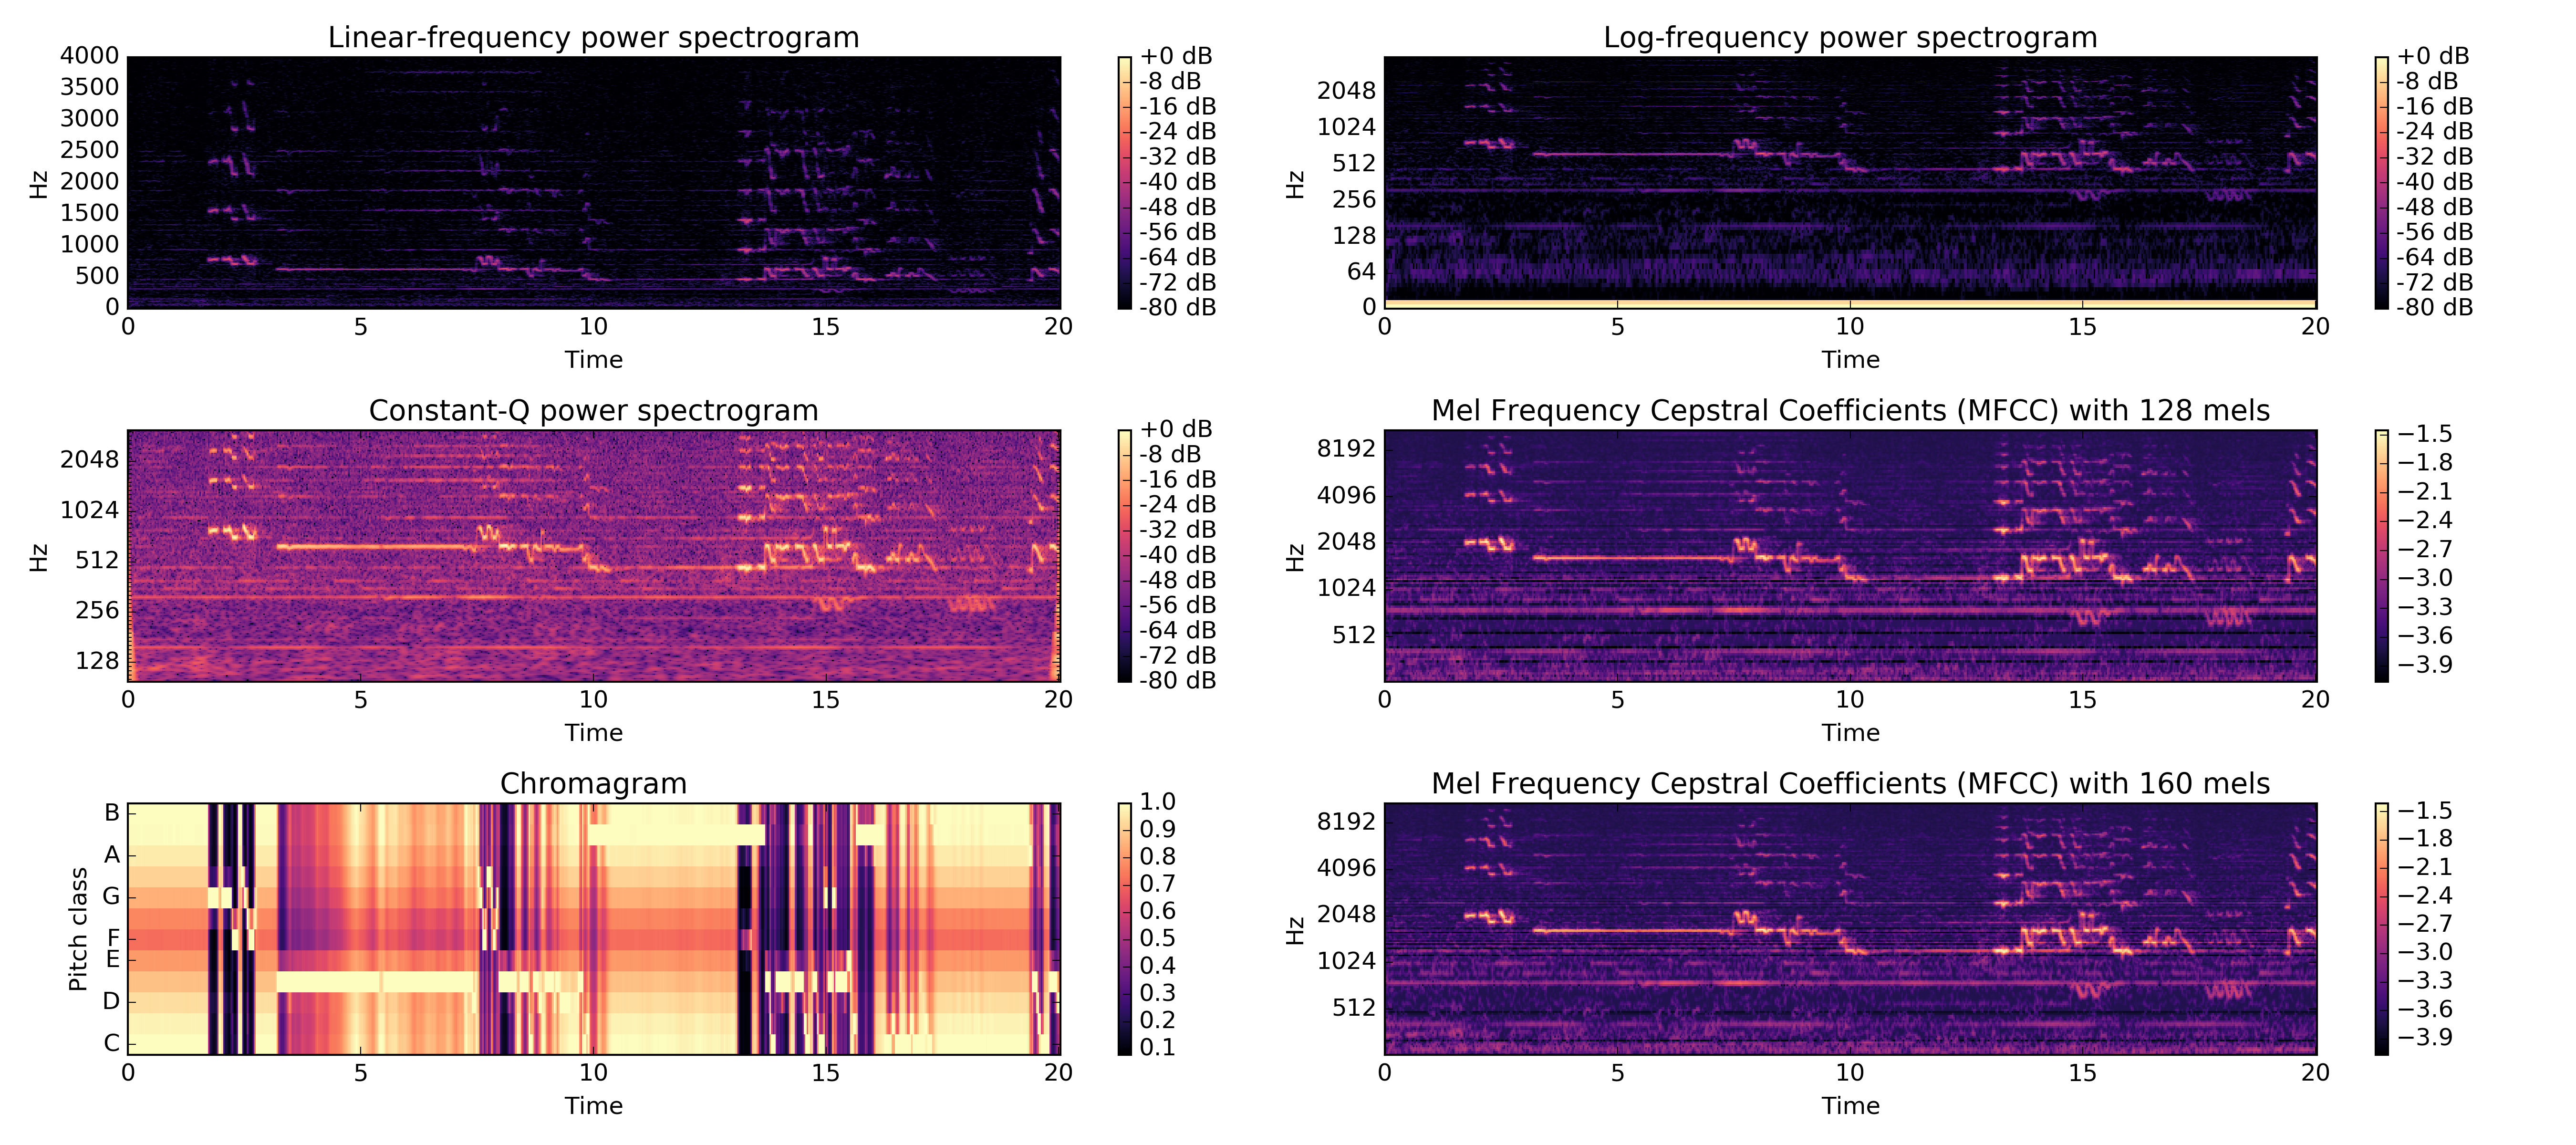
\includegraphics[scale=0.55]{audio_representations.png}
    \caption{Different Time-Frequency representations of the same fragment of carnatic music. In it, a t\=anpura plays a drone, while a flute plays a melody, responded by a violin in seconds 16 and 18.}
    \label{fig:representations}
  \end{sidewaysfigure}


  \subsubsection{Short-Term Fourier Transform (STFT)}

  The basic idea behind the STFT is, instead of performing a single Fourier transform for the whole waveform, to perform many transforms for small, overlapped chunks, a technique called {\it windowing} \cite[p.459]{musimathics}. The frequency resolution is given by the size of that window, and the time resolution by the overlapping factor. And since both parameters are independent from each other, it is possible to get arbitrary precission in both of them. The STFT also provides an inverse transform that allows a perfect reconstruction of the waveform (the exact details needed for a proper implementation can be seen in \cite[ch.10]{musimathics}). See the linear-frequency power spectrogram in Figure \ref{fig:representations} for an example of STFT.\\

  The STFT of a real, discrete analysis of size \(N\), with a window size \(W\) and an overlapping factor of \(O\), outputs a complex-valued matrix of heigth \(W\) and length \(\frac{ON}{W}\). The computational complexity of the STFT of a signal is in \(\mathcal{O}(ON log(W))\).

  \subsubsection{Log-STFT, CQT and MFCC}

  As we have seen, the discrete version of the Fourier transform ``carves up the spectrum of a sound into bins of constant bandwidth. But the sensitivity of the ear to frequency is logarithmic, that is, the ear's sensitivity to pitch diminishes with increasing pitch. From the ear's perspective, the DFT overspecifies high frequencies and underspecifies low frequencies''\cite[p.154]{musimathics}.\\

  This speaks against the criterium for a representation of conveying the relevant information in a convenient and accurate way: with a linear frequency scale, intervals that are perceived as identical have different sizes depending on the register; big portions of the representation convey rather irrelevant data and vice versa.\\

  One approach to overcome this problem is simply to map the vertical axis to a logarithmic scale and interpolate. See log-frequency power spectrogram (Log-STFT) in Figure \ref{fig:representations} for an example. But this doesn't actually solve any of the mentioned issues: the representation of the intervals still varies depending on the register; the lower end becomes very sparse and blurry, and the information in the higher end collapses and is hardly perceivable.\\

  A different approach involves analyzing the waveform with a different set of filters. As already seen, the set of filters that serves as basis for the STFT has the advantage of being linear and orthogonal. But this is mostly an advantage when performing real-time processing, and/or when a lossless signal reconstruction is needed. If none of those conditions apply, as in the case of the preprocessing stage of this thesis, other representations like the CQT and the MFCC may be considered:\\

  The Constant-Q transform (CQT) achieves a representation in which the vertical size of a musical interval remains constant across the whole frequency axis. But not only that: as noted in chapter \ref{about-car}, many musical systems are octave-neutral. The CQT captures this properties by arranging the positions of its filter bank to be repeated periodically every octave. In fact, in its original implementation\cite{cqt}, it is ``equivalent to a \(1/24^{th}\) bank of filters'', that, ``in addition to advantages for resolution, has the advantage that note identification, instrument recognition and signal separation can be done elegantly by a straightforward pattern recognition algorithm''\cite{cqt}. See the Constant-Q power spectrogram in Figure \ref{fig:representations} for an example.\\

  The Chromagram is a derived representation of the CQT: taking advantage of the fact that all the CQT filters are repeated every octave, it collapses all the octaves into one, showing the spectral intensity by pitch. The example of Figure \ref{fig:representations} was performed for 12 filters per octave, and shows clearly how the flute in the audio recording plays the notes G, F,  E${\flat}$ and B${\flat}$.\\


  The Mel Frequency Cepstral Coefficients (MFCC), on the other side, provide a more ``perceptually relevant representation''\cite{choi-robustness}, by  mapping `` the frequencies to the mel scale, which models human perception of changes in pitch, which is approximately linear below 1kHz and logarithmic above 1kHz.''\cite{haggblade}. Similarly to the CQT, it acts like a filter bank (with a more involved computation as further described in \cite{haggblade}), but as it can be seen in Figure \ref{fig:melscale}, the mel scale is not exactly logarithmic.\\

  \begin{figure}[h]
    \centering
    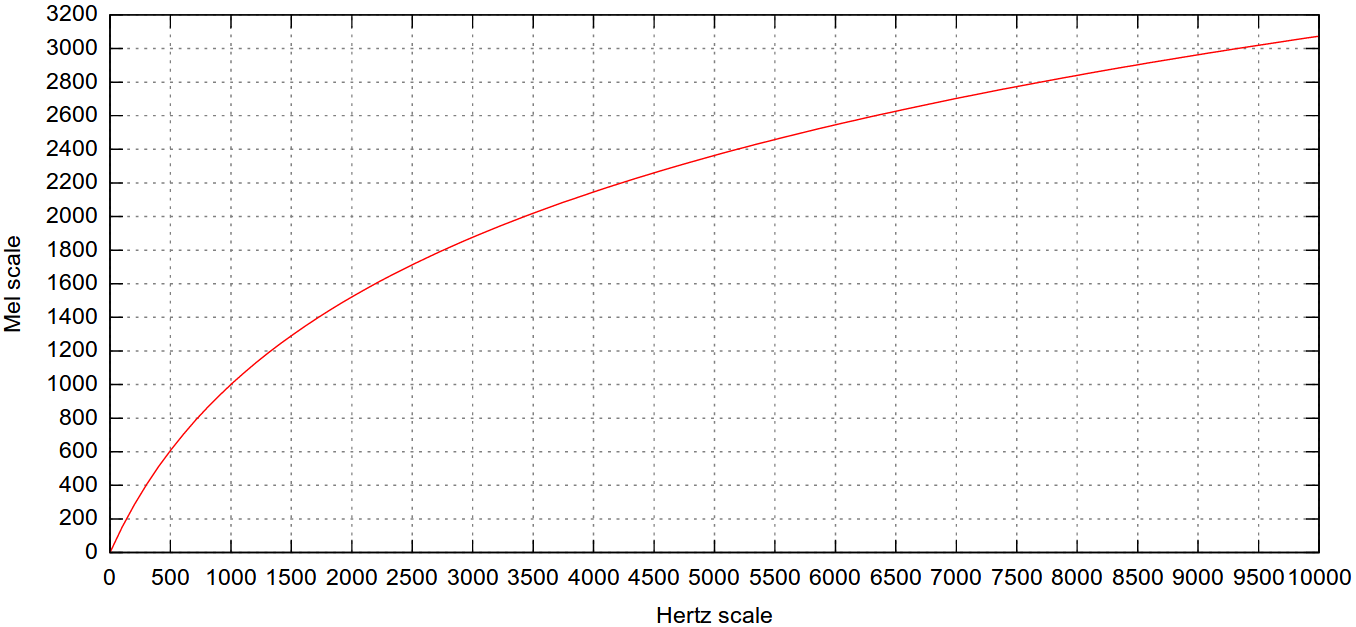
\includegraphics[scale=0.3]{mel_scale.png}
    \caption{A plot of the pitch mel scale versus Hertz scale}
    \label{fig:melscale}
  \end{figure}

  Since both the CQT and the MFCC representations are basically filter banks, their frequency domain is highly customizable, and they can be tweaked to convey the most convenient representation: in the LibROSA implementation, the CQT places the filters across the specified ambitus, with the specified interval resolution in filters per octave. The MFCC, on the other side, requires only the total number of filters to be used, and distributes them evenly across the mel scale. See the fifth section of the \texttt{3\_main\_pipeline.py} Python script for more details.\\

  Another interesting time-frequency representation, and the last one covered here is the one provided by the wavelet transform (WT). It is analogous to the Fourier transform, but instead of complex sinusoidals, the WT is based on wavelets, which are ``discrete families of functions obtained by dilations and translations of a finite number of well chosen moter functions.''\cite[1]{wavelets}. The emphasis is here on the ``well chosen'' attribute: as the sinusoidals, wavelets can also provide a linear orthogonal basis. This allows the nice computational properties as well as a lossless transformation, with the extra advantage of being both frequency and time localized. For that, the wavelet transform is considered ``more appropiate than Fourier series to represent the abrupt changes in non-stationary signals''\cite[1]{wavelets} and is used in many applications in the signal processing field.\\

  The Python script \texttt{6\_wavelet\_test.py} provides an implementation that calculates and plots the STFT and WT of selected .wav files, using the \texttt{PyWavelets} Python module\cite{pywt}. See Figures \ref{fig:rock_stft} and \ref{fig:rock_wt} for a possible output.



  \begin{sidewaysfigure}
    \centering
    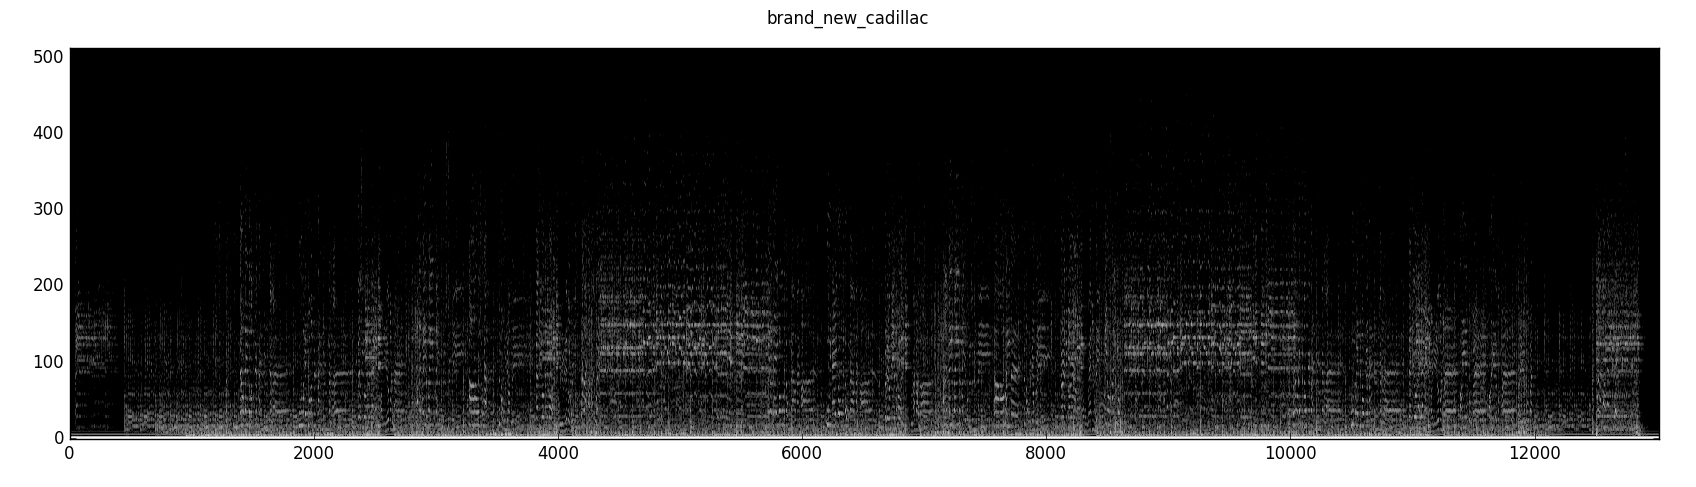
\includegraphics[width=\textheight*9/10,height=5.3cm]{brand_new_cadillac_stft.png}
    \caption{The STFT of a rock song, for a window size of 512, and an overlapping factor of 50\%.}
    \label{fig:rock_stft}
    \vspace{1.6cm}
    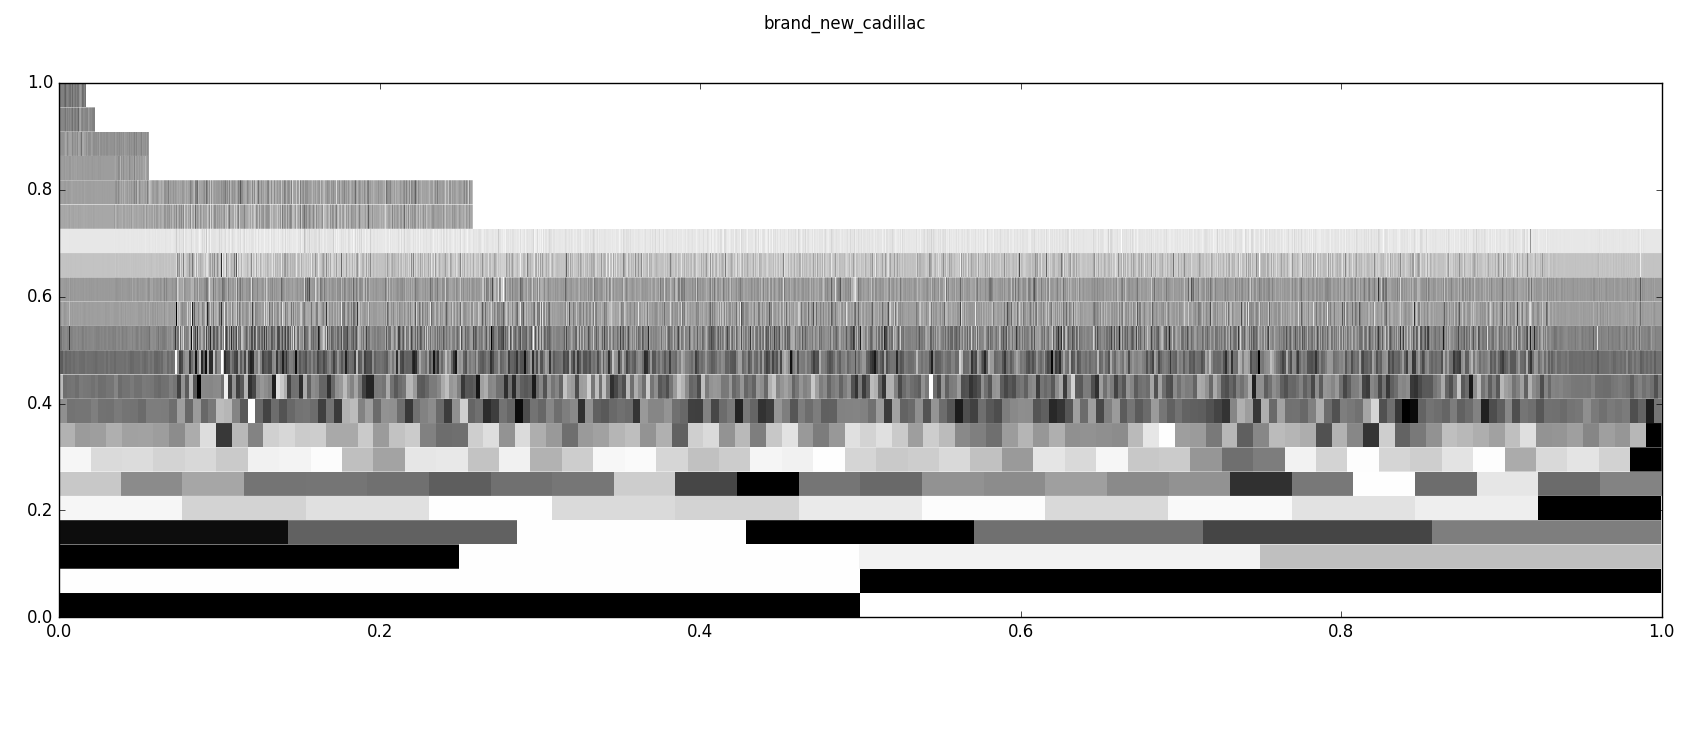
\includegraphics[width=\textheight*9/10,height=7cm]{brand_new_cadillac_wavelet.png}
    \vspace{-0.5cm}
    \caption{The wavelet transform of the same song, computed for the simplest Daubechies wavelet.}
    \label{fig:rock_wt}
  \end{sidewaysfigure}


  \section{Data Splitting} \label{datasplit}

  As explained in \label{crossvalidation}, the machine learning setups usually split the dataset into disjoint subsets. For that, it is important that the distribution of each resulting subset is as similar as possible to the distribution of the whole dataset. The problem that this poses is that, in many cases, a split that is similar with respect to some parameter becomes very different with respect to another.\\

  Take, for example, a set of 10 recordings that has to be fairly split into two equal subsets, having one recording with a duration of 9 hours, and the other 9 recordings being 1 hour long each. Taking apart the 9 hour recording for training and the rest for testing would be a perfect 50\%/50\% split with respect to the total duration, but an awful 90\%/10\% split with respect to the number of samples.\\

  To the best of my knowledge there is no general algorithm that performs a fair split for a given dataset in a fair an efficient way. This is usually a task that is undertaken by highly specialized curators, as in the case of the \(RRD_{CMD}\) dataset described in \ref{rrd_cmd}. For this thesis, I implemented two algorithms, described in the following sections.

  \subsubsection{First Approach}
  The splitting algorithm contained in the \texttt{4\_data\_split\_alt.py} Python script implements a heuristic that intends to promote a healthy balance between quantity and variety of the data in both resulting subsets. Given the set to split and the desired proportion, loops over the samples (sorted from smallest to biggest), performing the split by the given ratio until the proportion is achieved or surpassed. Such an approach could be useful only if the dataset has classes with very few samples and high duration variance.

  \subsubsection{Second Approach}

  This approach is followed by the \texttt{split\_labels} function in section seven of the \texttt{3\_main\_pipeline.py} Python script. This approach is based only in the number of recordings, and disregards the total duration of the resulting splitted subsets. It also includes further mechanisms to reject unfeasible splitting ratios or prevent splits resulting in any class having no representation.



  \section{Data Augmentation}\label{data-augm}

  Data augmentation is a form of regularization consisting in creating fake data and add it to the training set\cite[p.240]{goodfellow}.Further quoting, ``This approach is easiest for classification. A classifier needs to take a complicated, high dimensional input \(x\) and summarize it with a single category identity \(y\). This means that the main task facing a classifier is to be invariant to a wide variety of transformations. We can generate new \((x,y)\) pairs easily just by transforming the \(x\) inputs in our training set''.\\

  One of the problems that data augmentation can help to solve is class imbalance of the training set: when one class has more data than other (inter-class imbalance), or specific samples of one class are much bigger than others (intra-class imbalance),  random sampling from the training set will cause the model to overfit the most represented regions of the sample space. In order to solve this, there are four popular strategies:\\

  The most straightforward is to truncate the overrepresented classes. This is undesirable since data is the currency of machine learning, and should not be thrown away if it can be avoided.\\

  A more popular option is to balance the cost function by introducing a weight that is inversely proportional to the representativity of the given training sample. Since gradient descent bases its steps on the derivative of the cost function, this strategy naturally balances the learning process.\\

  Another option is to force data redundancy, by, for example, picking the same amount of information from every class each time. This will cause the data in the underrepresented classes to appear more often.\\

  Data augmentation works similarly to the data redundancy, but instead of reappearing identically, some transformation is applied to it. This transformation has to be chosen very carefully, as it has to be feasible for the problem domain in question. For instance, in an OCR application, linear transformations like stretching and scaling are feasible, but symmetrical rotations along the vertical axis are not.  This is well summarized in the following sentence: ``it is difficult to generate new fake data for a density estimation task unless we have already solved the density estimation problem''\cite[p.240]{goodfellow}: augmenting the data implies a somewhat explicit knowledge of the ground truth, but is {\it not} the ground truth (otherwise it wouldn't be necessary to perform any kind of machine learning since the problem would be solved). This is also why augmentation should never be applied to the validation or test datasets: testing on augmented data would assert whether the model has learned the augmentation paradigm and would skew the diagnose.

  \subsection{Augmentation Paradigms}

  For the r\=aga classification, I considered basically three strategies: noise injection, time stretching and frequency transposition.\\

  The first one is effective for speech recognition tasks\cite[p.241]{goodfellow}, and could be feasible here too, but I refrained from implementing it since most of the recordings that I checked are already very noisy.\\

  Frequency transposition is a feasible data augmentation paradigm for carnatic music, due to the fact that the fundamental frequency is an arbitrary factor, as already exposed in chapter \ref{about-car}.\\

  At first sight, time stretching seems feasible too: mildly changing the speed of a certain fragment shouldn't have a deep impact in its identity. But, as the temporal aspects do play a role in the definition of the r\=agas, this has to be done very carefully. Figure \ref{fig:chalan-stretch} illustrates that conveniently.

  \begin{figure}[h]
    \centering
    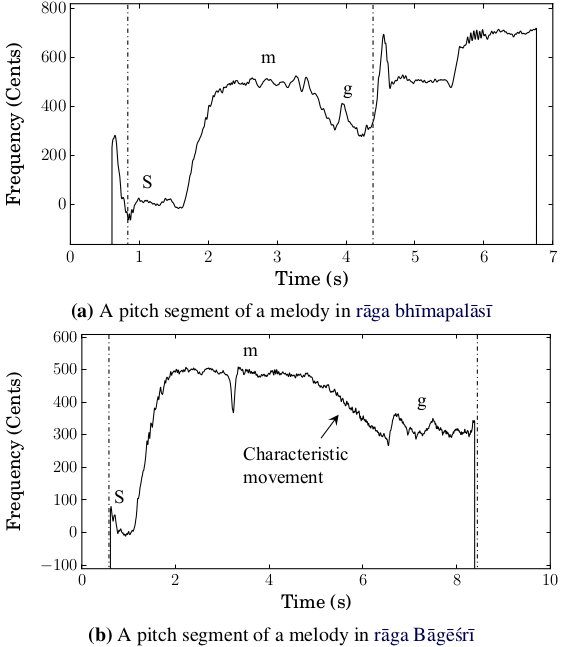
\includegraphics[scale=0.6]{chalan_stretch.png}
    \caption{Impact of temporal aspects in the r\=agas. Although the melodic transition in both r\=agas is made through the same set of svaras S, m, and g, in the same order, the characteristics of the transition regions in the melody and the duration of the svaras are different (from \cite[p.22]{gulati}).}
    \label{fig:chalan-stretch}
  \end{figure}


  \subsection{Implemented Augmentation}

  The \texttt{5\_data\_augmentation\_alt.py} Python script implements an augmentation algorithm that, by applying arbitrary transposition and stretching to given wav files, promotes intra-class and inter-class balance. The heuristic for the balance is very similar to the first approach explained in \ref{datasplit}.\\

  Note that the transposition and stretching factors are independent from each other. To achieve that, the script calls the third-party program \texttt{Rubber Band}\cite{rubberband}.


  \section{Data Feeding}\label{data_feeding}

  Once the required data has been loaded to the RAM, it has to be fed to the model. When performing stochastic gradient descent (explained in \ref{graddesc}), the model accepts data in the form of a batch, which is basically a vector of tensors. For that, the \texttt{3\_main\_pipeline.py} Python script implements two functions: \textt{get\_random\_batch} and \textt{cut\_sample\_to\_chunks}.\\

  The first one implements the functionality already explained as the ``data redundancy'' approach, in section \ref{data-augm}. This function is expected to be suitable for the training phase, since it provides a fair inter-class and intra-class balance:  for each element of the batch, all the classes have the same random probability of being represented, and the same happens for all the samples within a class. The sample is also expected to be fairly represented in the long run, since the position of the window extracted from it is also drawn from a random uniform distribution.\\

  The second one cuts a given sample of arbitrary size into chunks of the specified size, discarding the last chunk if it is smaller than the rest. This paradigm is more suitable for validation and testing purposes, since it allows an efficient and flexible implementation of voting mechanisms (voting only makes sense among chunks of the same sample, more details in section \ref{errormetrics}), and it doesn't matter that all the chunks belong to the same class, since the whole subset will be processed and taken into account for the error metrics.



  \section{Model Implementation}

  In every supervised learning setup, there is a set of tasks that has to be repeated almost identically every time, regardless of the exact model or parameters being used. Specialized machine learning libraries like TensorFlow, described later, help to take care of many of these tasks.\\

  On a higher level, the tasks concerning the implementation of the model can be encapsulated into three functional groups: definition, training and testing. The software patterns resulting from that encapsulation are also described in this section.\\

  Visualizing the results can be also very helpful for debugging the model and interpreting its results. TensorBoard, explained at the end of the section, provides good functionality for that.

  \subsection{About TensorFlow}

  TensorFlow is an open source software library for numeric computation developed by Google\cite{tflow}. Originally developed for conducting machine learning and deep neural networks research, it makes very easy to work with GPUs, and has a broad built-in support for machine-learning related functionality. Tensorflow organizes the computation using data flow graphs: ``nodes in the graph represent mathematical operations, while the graph edges represent the multidimensional data arrays (tensors) communicated between them''\cite{tflow}.

  \subsubsection{Lifecycle and Namespaces}

  Most of the functionality of TensorFlow is written in C++. Therefore, the Python programs using TensorFlow have two distinct parts: building the computational graph (which has to be compiled into C++ and is statically typechecked) and running it.\\

  In order to access the previously compiled nodes, TensorFlow provides a global namespace system, which can be visited with the \texttt{get\_tensor\_by\_name} function or by applying Python's \texttt{with} context manager to the corresponding object (usually a \texttt{Graph} instance, a \texttt{Session} instance or a call to the \texttt{tf.name\_scope} function).



  \subsubsection{Building the Graph}

  The dataflow in a \texttt{Graph} usually starts with a \texttt{constant}, a \texttt{Variable} or a \texttt{placeholder} nodes, which are designed to contain tensors. The contents of the constant are statically bound when compiling the graph and cannot change. The contents of the Variable are more flexible: they can be updated while running the graph but have to be initialized for a fixed shape at the beginning of the session. The placeholders are the most flexible of all, since they don't have to be initialized: At the moment of evaluating the contents of a node, the mapping from every placeholder involved in the computation to its corresponding data has to be provided in the form of a dictionary called the \texttt{feed\_dict}. This matches very well the functionality described in section \ref{data_feeding}.\\

  The connection from one node to another is expressed by passing the existing node as an argument to the constructor of the following node. Mirroring the functionality of NumPy, TensorFlow provides support for most arithmetic and memory operations, as well as many machine-learning related computations, so most of the mainstream models (like neural networks) are very straightforward to implement. As an example of how to build a graph, see the function \texttt{make\_custom\_graph} in the \texttt{3\_main\_pipeline.py} Python script.\\

  Among the most specialized built-in nodes are the optimizers: when an optimizer is positioned in the graph (usually by passing a cost function to it), TensorFlow traverses all its underlying nodes, attaching the corresponding optimization operation to it (for the gradient descent optimizers, this is the backpropagation algorithm), and keeping track of the variables that it finds. Then, when its \texttt{minimize} method is run, the optimization is computed through the attached nodes, and the tracked variables are updated with the optimized values. See \cite[p.212]{goodfellow} for a more detailled explanation.


  \subsubsection{Running the Graph}

  The process of running the previously compiled graph is managed by an instance of the \texttt{Session} class, via its \texttt{run} method, which accepts a node or list of nodes as its first argument. Calling run for a node will traverse down the graph until reaching the initial nodes. Then, followning the topological ordering of the graph, the computation is propagated forward, until all the values for the required nodes are eventually calculated and returned by the method.\\

  The function \texttt{run\_training}  in the \texttt{3\_main\_pipeline.py} Python script illustrates how this can be done. Note that if any of the initial nodes is a placeholders, a value for it has to be provided in the feed\_dict.


  \subsection{Model Definition}

  All the models defined in the \texttt{3\_main\_pipeline.py} Python script are expected to receive a batch of data with its corresponding batch of labels, and some extra hyperparameters like, for example, the dropout rate to be applied. Then, they use their parameters, stored in variables, to propagate the given data and produce a hypothesis in the form of a logit vector, which is returned together with the L2 loss for all the model's parameters excluding the bias.\\

  If the model is defined in accordance to this interface, the \texttt{make\_custom\_graph} function will be able to integrate it successfully. This function takes care of creating a graph with the following functionality, common to every model:

  \begin{itemize}
  \item creates the placeholders for the different input batches and hyperparameters
  \item integrates the specified model and defines the cost function for it, with the given L2 regularization hyperparameter.
  \item instantiates the specified optimizer with the given learning rate, and sets it to optimize the cost function above mentioned.
  \item implements some basic metrics like correct predictions and mean accuracy of the given batch.
  \end{itemize}

  The function returns then the whole graph, as well as two dictionaries; one with the input nodes and one with the outputs.

  \subsection{Model Training}

  Following the idea of the  \texttt{make\_custom\_graph} function,  \texttt{run\_training} intends to provide a simple yet highly customizable interface to the user. Its parameter list is the following:

  \lstset{language=Python}
  \lstset{basicstyle=\footnotesize}
  \begin{lstlisting}

    def run_training(train_ddict, cv_ddict, test_ddict,
    model, optimizer_manager,
    batch_size, chunk_size, l2rate_fn, dropout_fn,
    log_path,
    batch_freq=100, cv_freq=500,
    cv_voting_size=1, test_voting_size=1,
    max_steps=float("inf"),
    extra_info="",
    normalize_chunks=True,
    max_gpu_memory_fraction=1)
  \end{lstlisting}

  Most of its parameters are self-explanatory: this function instantiates the graph for the given model, optimizer and hyperparameters. Then starts the session, and then runs the training loop. Every iteration loads a batch provided by \textt{get\_random\_batch} and trains the model by running the optimizer. Also, the statistics for the training and validation steps are output with the specified frequency.\\

  The \texttt{OptimizerManager} class is simply a wrapper for the existing tensorflow optimizers, to allow a better integration in the graph. Note that the regularization, dropout and learning rate hyperparameters are to be passed as functions that accept the current training step as parameter. This allows to model arbitrarily complex behaviors (like, for example, learning rate decay) without any structural changes in the code.

  \subsection{Model Testing}

  Every \texttt{cv\_freq} steps, the whole validation set is evaluated. This is done by converting all of its records to batches with \texttt{cut\_sample\_to\_chunks}, feeding the batches to the graph (by the specified \texttt{cv\_voting\_size}) and storing the results into an instance of the \texttt{ConfusionMatrix} class, which keeps track of the results and provides functionality for calculating the total and the by-class accuracy.\\

  When the whole subset has been tested, it is possible to create and export a plot of the matrix with the \texttt{add\_confmatrix} method of the \texttt{TensorBoardLogger} class.

  \subsection{Visualization with TensorBoard}  \label{tb-visualization}

  TensorBoard is a suite of visualization tools designed to run on a HTTP server, that can be then visited by a web browser. It provides real-time information on the implemented model, by showing its computational graph as well as the functions, images, audio files and/or histograms that it may generate. For that, the server visits a log directory that has to be specified when it starts with the \texttt{--logdir} flag, and serves to a given IP address (\texttt{localhost:6006} by default).\\

  This log directory contains a set of protocol buffers\cite{protobufs}, which are basically extensible strings that contain data like functions, images, audio files, as well as the metadata attached to them like date and title. This buffers are generated and interactively expanded by the \texttt{tf.summary.FileWriter}, and the contents are represented in TensorFlow by the \texttt{tf.Summary} objects.\\

  The \texttt{TensorBoardLogger} class in the \texttt{3\_main\_pipeline.py} Python script provides an implementation that outputs functions and matrix plots to the specified log directory.\\

  In some cases, the computer holding the log files is only accessible via SSH and prevents visiting the TensorBoard HTTP server. In that case, SSH tunneling can be performed: The following command forwards TensorBoard to \texttt{localhost:16006}, assuming it was started with the default IP address:\\
  \texttt{ssh -p <PORT> <USER>@<SERVER> -N -f -L localhost:16006:localhost:6006}
